\documentclass{beamer}
\graphicspath{{images/}}

\title{Intro to Git}
\date{}

\begin{document}

\frame{\titlepage}

\begin{frame}
	\frametitle{Plan}
	\begin{itemize}
		\item{Intro to Version Control}
		\item{Getting Started}
		\item{Git Basics}
		\item{Branches in Git}
		\item{Git Reset in Detail}
	\end{itemize}
\end{frame}

% Section 1: Into to Version Control

\begin{frame}
	\frametitle{Intro to Version Control}
	\begin{itemize}
		\item{System that records changes to a file or set of files over time (VCS)}
		\item{Can recall specific versions at a later time}
		\item{Can revert individual files or even the entire project to a previous state}
		\item{Can compare changes in files over time}
		\item{Can see who modified something and when}
		\item{Does the very efficiently}
		\item{Set of all versions of all files called a repository}
	\end{itemize}
\end{frame}

\begin{frame}
	\frametitle{Local VCS}
	\begin{itemize}
		\item{Simple database containing all changes to file under version control}
	\end{itemize}
	\begin{figure}
		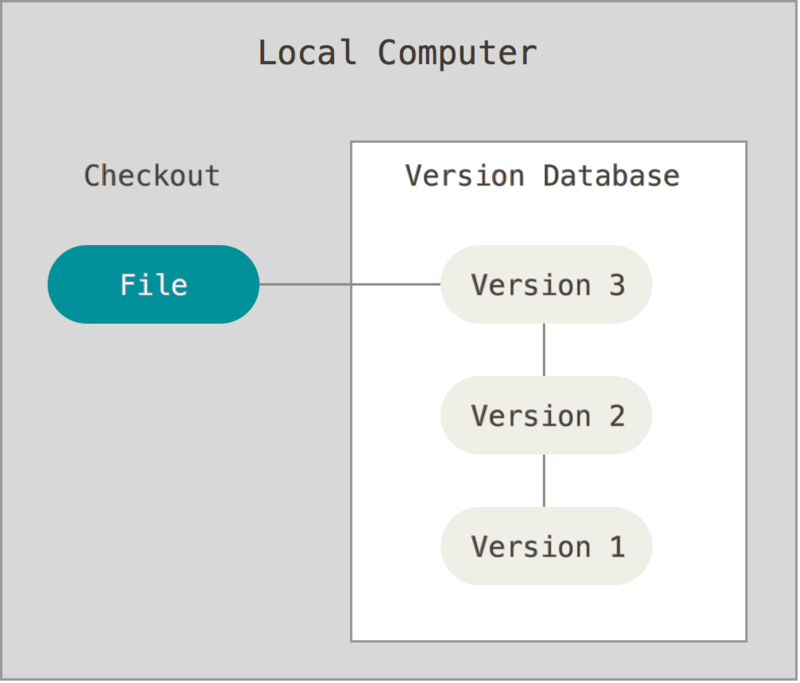
\includegraphics[scale=0.25]{Local_VCS-0.png}
	\end{figure}
\end{frame}

\begin{frame}
	\frametitle{Centralised VCS}
	\begin{itemize}
		\item{Used to collaborate with other developers}
		\item{Single server contains all the versioned files}
		\item{Clients check out snapshots from the server}
	\end{itemize}
	\begin{figure}
		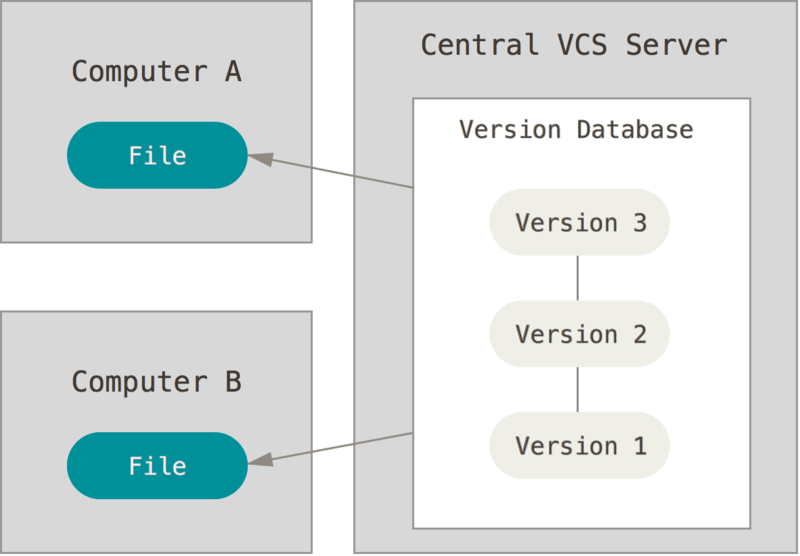
\includegraphics[scale=0.25]{Centralised_VCS-0.png}
	\end{figure}
\end{frame}

\begin{frame}
	\frametitle{Distributed VCS}
	\begin{itemize}
		\item{Each client fully mirrors the the repository}
		\item{Allows direct collaboration between developers}
	\end{itemize}
	\begin{figure}
		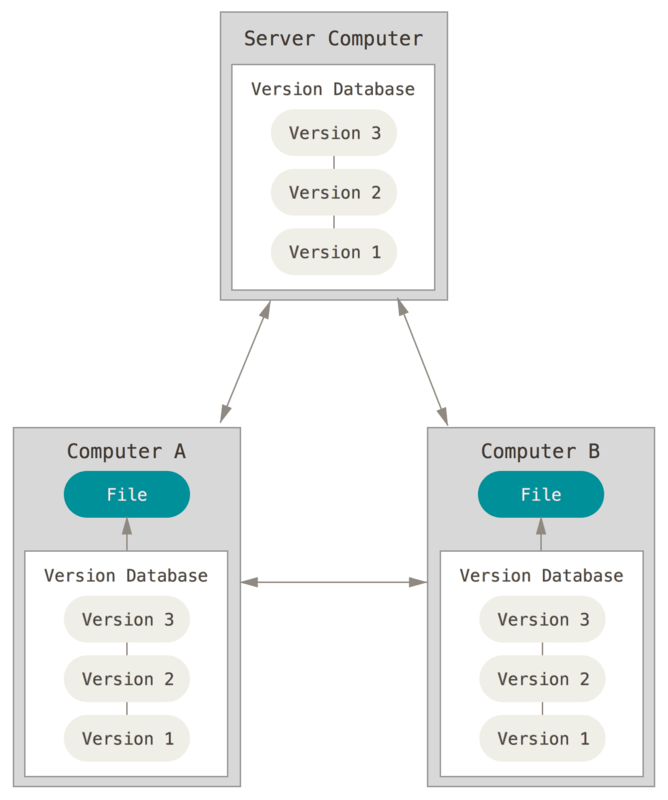
\includegraphics[scale=0.25]{Distributed_VCS-0.png}
	\end{figure}
\end{frame}

% Section 2: Getting Started

\begin{frame}
	\frametitle{A Short History of Git}
	\begin{itemize}
		\item{Created by Linus Torvalds in 2005 for Linux kernel development}
		\item{The goals for Git were:}
		\begin{itemize}
			\item{Speed}
			\item{Simple design}
			\item{Able to handle large projects}
			\item{Fully distributed}
			\item{Very good support for non-linear development}
		\end{itemize}
	\end{itemize}
\end{frame}

\begin{frame}
	\frametitle{Differences}
	\begin{itemize}
		\item{Store initial file version and each change over time}
	\end{itemize}
	\begin{figure}
		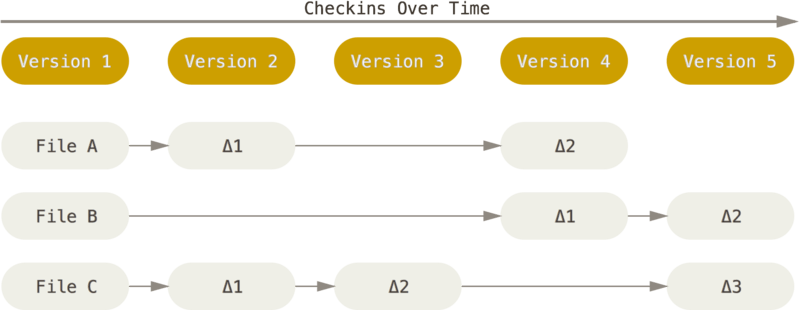
\includegraphics[scale=0.25]{Differences-0.png}
	\end{figure}
\end{frame}

\begin{frame}
	\frametitle{Snapshots}
	\begin{itemize}
		\item{Every time you commit (save) the project state, a new snapshot of is made}
		\item{A snapshot is a "picture" of all the files in the repo}
		\item{Files that haven't changed aren't saved for efficiency}
	\end{itemize}
	\begin{figure}
		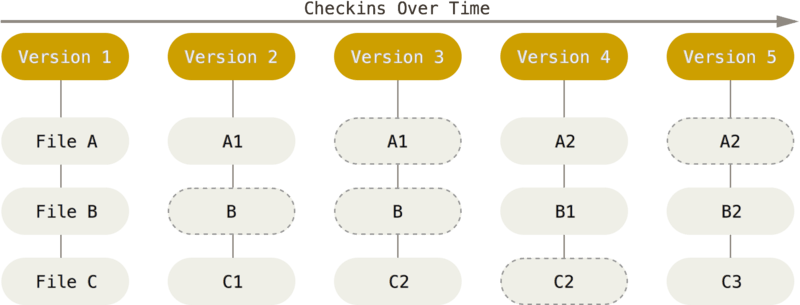
\includegraphics[scale=0.25]{Snapshots-0.png}
	\end{figure}
\end{frame}

\begin{frame}
	\frametitle{Almost everything in Git is local}
	\begin{itemize}
		\item{Most operations in Git only affect your local copy of the repo}
		\item{Very rarely need to go onto the network}
		\item{No network latency}
		\item{Can work offline}
	\end{itemize}
	\begin{figure}
		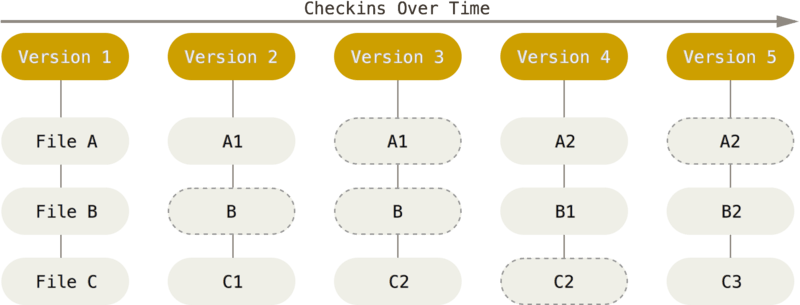
\includegraphics[scale=0.25]{Snapshots-0.png}
	\end{figure}
\end{frame}

\begin{frame}
	\frametitle{Git has built-in integrity checking}
	\begin{itemize}
		\item{Everything stored in Git is check-summed}
		\item{Changing something changes the checksum and the history}
		\item{Git is able to detect any file corruption or modification}
		\item{24b9da6552252987aa493b52f8696cd6d3b00373}
		\item{SHA-1 hash (40-char hex string)}
	\end{itemize}
\end{frame}

\begin{frame}
	\frametitle{The Three States}
	\begin{itemize}
		\item{One of the most important things in Git}
		\item{Files in your repository exist in one of three states}
		\item{Committed: Safely stored in your local database}
		\item{Modified: Changed a file but not committed it yet}
		\item{Staged: Marked a modified file to go in the next commit snapshot}
	\end{itemize}
	\begin{figure}
		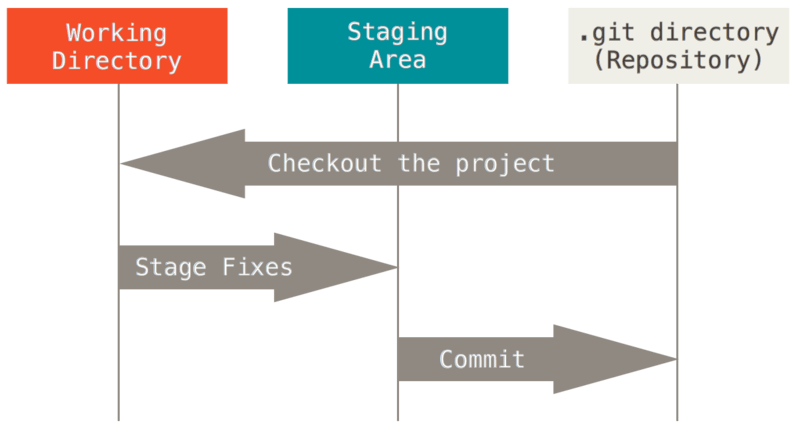
\includegraphics[scale=0.25]{The_Three_States-0.png}
	\end{figure}
\end{frame}

\begin{frame}
	\frametitle{The Three States}
	\begin{itemize}
		\item{The .git directory is where Git stores the snapshots}
		\item{The working tree is a single snapshot of the repository}
		\item{Uncompressing a snapshot from .git is called "checking out"}
		\item{The staging area stores information about what goes into the next commit}
	\end{itemize}
\end{frame}

\begin{frame}
	\frametitle{Development Cycle}
	\begin{itemize}
		\item{1. Modify files in working tree}
		\item{2. Stage some of the modified files}
		\item{3. Do a commit, saving the contents of the staging area into a new snapshot}
	\end{itemize}
\end{frame}

\begin{frame}
	\frametitle{Installing Git}
	\begin{itemize}
		\item{Available on Linux, Windows, Mac}
		\item{Package managers or from source at https://github.com/git/git/releases}
	\end{itemize}
\end{frame}

\begin{frame}
	\frametitle{First Time Configuration}
	\begin{itemize}
		\item{Configuration in git is done with the \textbf{git config} command}
		\item{This command allows you to get and set configuration variables}
		\item{These variables can be stored in three different places}
		\item{/etc/gitconfig file: System-wide values, use --system switch}
		\item{\textasciitilde{}/.gitconfig or \textasciitilde{}/.config/git/config file: This user only, use --global switch}
		\item{.git/config file: This repository only, no switch required}
	\end{itemize}
\end{frame}

\begin{frame}
	\frametitle{First Time Configuration}
	\begin{itemize}
		\item{\textbf{git config \texttt{-{}-}global user.name "Sam Caulfield"}}
		\item{\textbf{git config user.email "sam.caulfield@movidius.com"}}
		\item{\textbf{git config \texttt{-{}-}system core.editor "vim"}}
		\item{Precedence: Per Repository \textgreater{} Per User \textgreater{} System}
		\item{Show configuration settings with \textbf{git config \texttt{-{}-}list}}
		\item{Show just one configuration option with \textbf{git config user.name}}
	\end{itemize}
\end{frame}

\begin{frame}
	\frametitle{Getting help}
	\begin{itemize}
		\item{\textbf{git help \textless{}verb\textgreater{}}}
		\item{\textbf{git \textless{}verb\textgreater{} \texttt{-{}-}help}}
		\item{\textbf{man git-\textless{}verb\textgreater{}}}
		\item{https://git-scm.com/book/en/v2/}
	\end{itemize}
\end{frame}

% Section 3: Git Basics

\begin{frame}
	\frametitle{Getting a Git Repository}
	\begin{itemize}
		\item{Two main ways: create one or copy one}
		\item{To create one: \textbf{git init} or \textbf{git init MyRepo}}
		\item{To copy one: \textbf{git clone https://github.com/libgit2/libgit2}}
	\end{itemize}
\end{frame}

\begin{frame}
	\frametitle{Recording Changes to the Repository}
	\begin{itemize}
		\item{Need to make changes and commit snapshots}
		\item{Files in the working directory are either tracked or untracked}
		\item{Tracked: Present in the previous snapshot}
		\item{Untracked: Not present in the previous snapshot or in the staging area}
		\item{Tracked files can be unmodified, modified, or staged}
	\end{itemize}
	\begin{figure}
		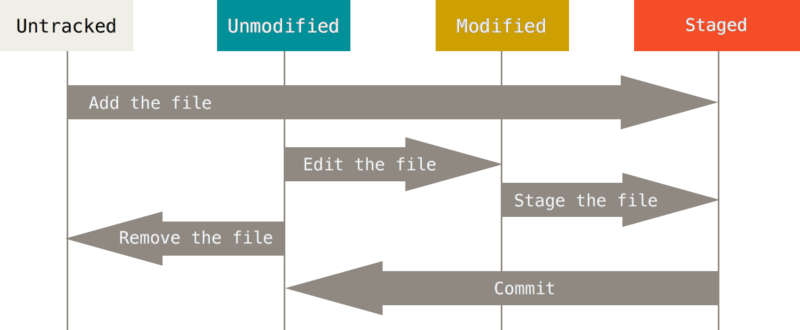
\includegraphics[scale=0.37]{Recording_Changes_to_the_Repository-0.png}
	\end{figure}
\end{frame}

\begin{frame}
	\frametitle{Checking the Status of Files}
	\begin{itemize}
		\item{Done with the \textbf{git status} command}
	\end{itemize}
	\begin{figure}
		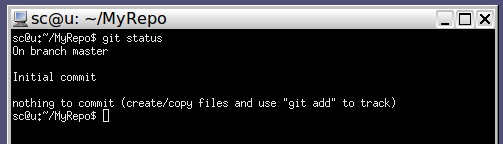
\includegraphics[scale=0.50]{Checking_the_Status_of_Files-0.png}
	\end{figure}
	\begin{figure}
		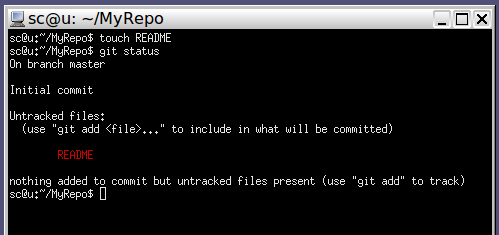
\includegraphics[scale=0.50]{Checking_the_Status_of_Files-1.png}
	\end{figure}
\end{frame}

\begin{frame}
	\frametitle{Tracking New Files}
	\begin{itemize}
		\item{Done with the \textbf{git add} command}
	\end{itemize}
	\begin{figure}
		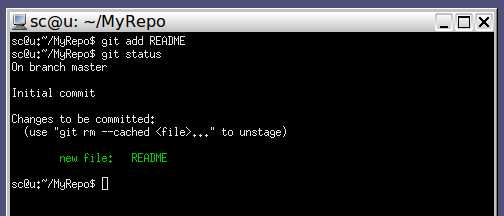
\includegraphics[scale=0.50]{Tracking_New_Files-0.png}
	\end{figure}
\end{frame}

\begin{frame}
	\frametitle{Staging Modified Files}
	\begin{figure}
		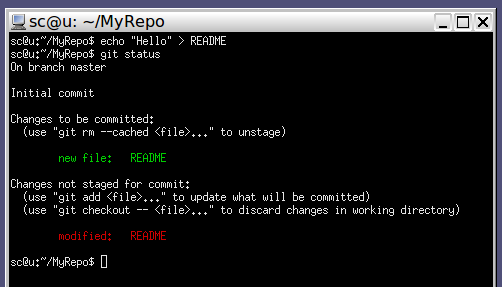
\includegraphics[scale=0.60]{Staging_Modified_Files-0.png}
	\end{figure}
\end{frame}

\begin{frame}
	\frametitle{Staging Modified Files}
	\begin{itemize}
		\item{Done with the \textbf{git add} command}
		\item{\textbf{git add \texttt{-{}-}patch} can be used to stage parts of files}
	\end{itemize}
	\begin{figure}
		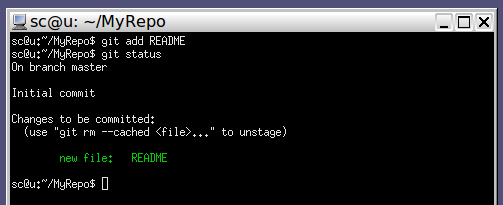
\includegraphics[scale=0.60]{Staging_Modified_Files-1.png}
	\end{figure}
\end{frame}

\begin{frame}
	\frametitle{Short Status}
	\begin{itemize}
		\item{\textbf{git status -s} provides a less verbose status report}
		\item{Untracked files have a ?? next to them}
		\item{New files that have been added to the staging area have an A}
		\item{Modified files have an M, etc.}
		\item{Left column: index, right column: working directory}
	\end{itemize}
	\begin{figure}
		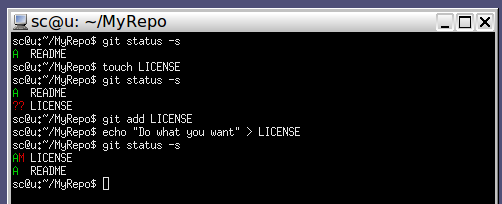
\includegraphics[scale=0.62]{Short_Status-0.png}
	\end{figure}
\end{frame}

\begin{frame}
	\frametitle{Ignoring Files}
	\begin{itemize}
		\item{The working directory can easily become full of files you don't want to version}
		\item{.o, .swp, .log, etc.}
		\item{They can clog up the output of \textbf{git status}}
		\item{List unwanted file types in a .gitignore file in the repository}
		\item{\textbf{echo *.o \textgreater{} .gitignore}}
		\item{Can perform simple pattern matching: doc/**/*.pdf}
	\end{itemize}
\end{frame}

\begin{frame}
	\frametitle{Viewing Staged and Unstaged Changes}
	\begin{itemize}
		\item{What have I changed but not staged?}
		\item{What have I staged that I am about to commit?}
		\item{Use the \textbf{git diff} command}
		\item{This shows what's changed in the working directory that isn't staged}
	\end{itemize}
	\begin{figure}
		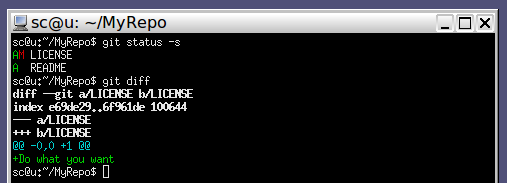
\includegraphics[scale=0.62]{Viewing_Staged_and_Unstaged_Changes-0.png}
	\end{figure}
\end{frame}

\begin{frame}
	\frametitle{Viewing Staged and Unstaged Changes}
	\begin{itemize}
		\item{To view what's new in the staging area use \textbf{git diff --staged}}
	\end{itemize}
	\begin{figure}
		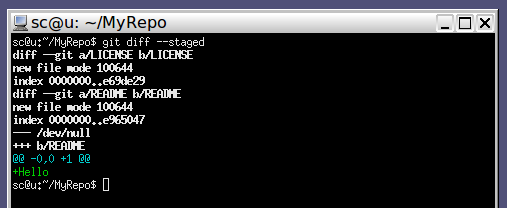
\includegraphics[scale=0.62]{Viewing_Staged_and_Unstaged_Changes-1.png}
	\end{figure}
\end{frame}

\begin{frame}
	\frametitle{Committing Your Changes}
	\begin{itemize}
		\item{Committing creates a new snapshot in the project history}
		\item{The snapshot is the previous snapshot + the staging area changes}
		\item{Anything left in the working directory and not in the staging area isn't included}
		\item{Use the \textbf{git commit} command}
	\end{itemize}
	\begin{figure}
		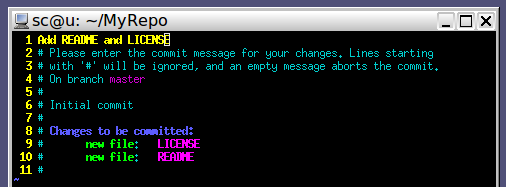
\includegraphics[scale=0.62]{Committing_Your_Changes-0.png}
	\end{figure}
\end{frame}

\begin{frame}
	\frametitle{Committing Your Changes}
	\begin{itemize}
		\item{Saving and closing the editor confirms the commit}
		\item{Alternatively, you can use \textbf{git commit -m "Add README and LICENSE"}}
		\item{Can skip staging with \textbf{git commit -a}}
	\end{itemize}
	\begin{figure}
		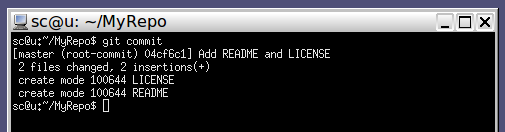
\includegraphics[scale=0.62]{Committing_Your_Changes-1.png}
	\end{figure}
\end{frame}

\begin{frame}
	\frametitle{Removing Files from the Repository}
	\begin{itemize}
		\item{Use the \textbf{git rm} command}
	\end{itemize}
	\begin{figure}
		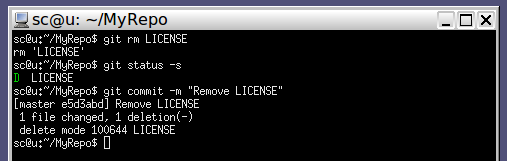
\includegraphics[scale=0.62]{Removing_Files_from_the_Repository-0.png}
	\end{figure}
	\begin{itemize}
		\item{Similarly, \textbf{git mv} can be used to move files}
	\end{itemize}
\end{frame}

\begin{frame}
	\frametitle{Viewing the Commit History}
	\begin{itemize}
		\item{Use the \textbf{git log} command}
	\end{itemize}
	\begin{figure}
		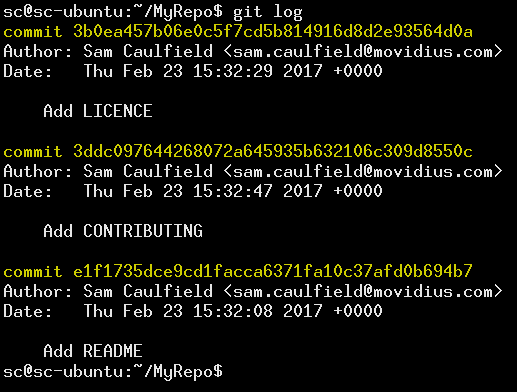
\includegraphics[scale=0.6]{Viewing_the_Commit_History-0.png}
	\end{figure}
\end{frame}

\begin{frame}
	\frametitle{Viewing the Commit History}
	\begin{itemize}
		\item{Can control the output of \textbf{git log}}
		\item{-p: Show diffs in each commit}
		\item{-1: Limit output to last 1 commit}
	\end{itemize}
	\begin{figure}
		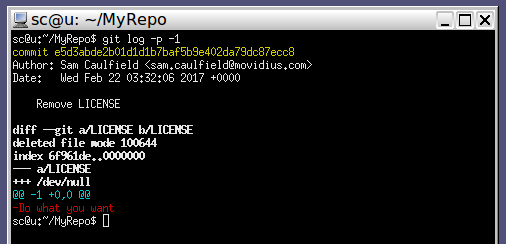
\includegraphics[scale=0.6]{Viewing_the_Commit_History-1.png}
	\end{figure}
\end{frame}

\begin{frame}
	\frametitle{Viewing the Commit History}
	\begin{itemize}
		\item{Keep logs to one line each: \textbf{git log \texttt{-{}-}pretty=oneline}}
	\end{itemize}
	\begin{figure}
		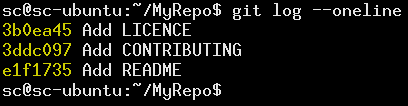
\includegraphics[scale=0.6]{Viewing_the_Commit_History-2.png}
	\end{figure}
\end{frame}

\begin{frame}
	\frametitle{Viewing the Commit History}
	\begin{itemize}
		\item{Restrict output based on time: \textbf{git log \texttt{-{}-}since=1.day}}
		\item{See what commits modified a string: \textbf{git log -Ssomestring}}
		\item{Filter by author: \textbf{git log \texttt{-{}-}author}}
		\item{Filter by commit message content: \textbf{git log \texttt{-{}-}grep}}
	\end{itemize}
\end{frame}

\begin{frame}
	\frametitle{Undoing Things}
	\begin{itemize}
		\item{You can amend a commit if you forgot something}
		\item{Use \textbf{git commit \texttt{-{}-}amend}}
		\item{Takes your staging area and adds it to the most recent commit}
		\item{Results in a single commit: original + changes}
	\end{itemize}
\end{frame}

\begin{frame}
	\frametitle{Unstaging Staged Files}
	\begin{itemize}
		\item{Use the \textbf{git reset HEAD \textless{}file\textgreater{}} command}
		\item{This removes the file from the staging area}
	\end{itemize}
\end{frame}

\begin{frame}
	\frametitle{Unmodifying Modified Files}
	\begin{itemize}
		\item{In Git, "unmodifying" means resetting a file back to the previous snapshot}
		\item{Use the \textbf{git checkout \texttt{-{}-} \textless{}file\textgreater{}} command}
		\item{Warning: since uncommitted changes are being removed, the changes will be lost}
	\end{itemize}
\end{frame}

\begin{frame}
	\frametitle{Aliases}
	\begin{itemize}
		\item{Can be used to shorten Git commands}
		\item{Allows you to type "git st" instead of "git status", etc.}
		\item{\textbf{git config --global alias.st status}}
		\item{\textbf{git config --global alias.unstage 'reset HEAD'}}
	\end{itemize}
	\begin{figure}
		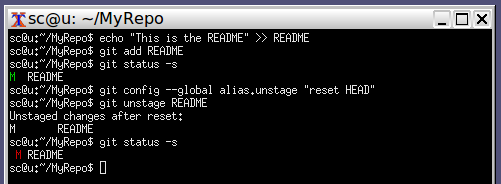
\includegraphics[scale=0.62]{Aliases-0.png}
	\end{figure}
\end{frame}

% Section 4: Branches in Git

\begin{frame}
	\frametitle{Branches in Git}
	\begin{itemize}
		\item{Branching: Diverge from the main line of development}
		\item{Continue working on a different "line" of development}
		\item{Can merge back into the main line when complete}
		\item{One of Git's best features}
	\end{itemize}
\end{frame}

\begin{frame}
	\frametitle{How Git Branches Work}
	\begin{itemize}
		\item{When you make a commit, Git stores a commit object}
		\item{The commit object stores a pointer to the snapshot of the staged content}
		\item{Each commit also points to its parent, the one that came before it}
		\item{Only the root commit (the first in the repository) doesn't have a parent}
		\item{Some commits can have multiple parents in the case of merge commits}
	\end{itemize}
\end{frame}

\begin{frame}
	\frametitle{How Git Branches Work}
	\begin{figure}
		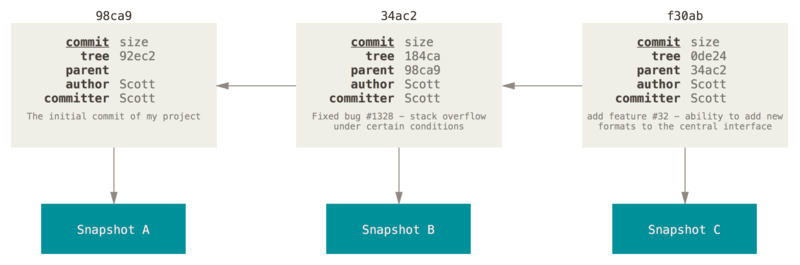
\includegraphics[scale=0.40]{How_Git_Branches_Work-0.png}
	\end{figure}
\end{frame}

\begin{frame}
	\frametitle{How Git Branches Work}
	\begin{figure}
		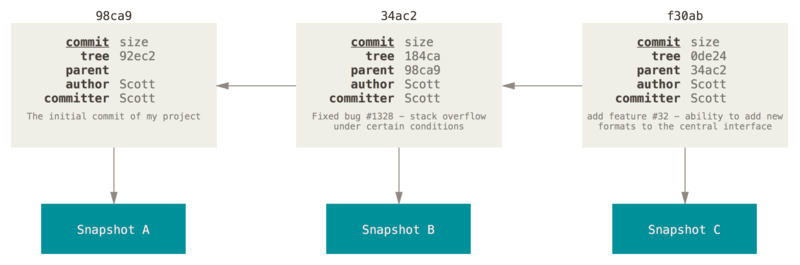
\includegraphics[scale=0.30]{How_Git_Branches_Work-0.png}
	\end{figure}
	\begin{itemize}
		\item{A branch in Git is simply a pointer to one of these commits}
		\item{The pointer is moveable}
		\item{In Git, the default branch is called \textbf{master}}
		\item{The branch pointer points to the most recent commit on the branch history}
		\item{When you commit on a branch, the branch pointer automatically moves forward}
	\end{itemize}
\end{frame}

\begin{frame}
	\frametitle{How Git Branches Work}
	\begin{figure}
		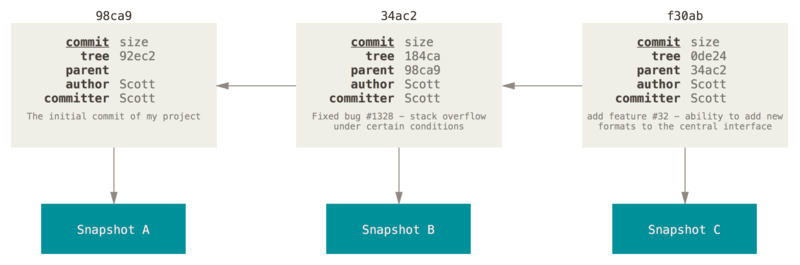
\includegraphics[scale=0.30]{How_Git_Branches_Work-0.png}
	\end{figure}
	\begin{itemize}
		\item{A branch in Git is simply a pointer to one of these commits}
		\item{The pointer is moveable}
		\item{In Git, the default branch is called \textbf{master}}
		\item{When you commit on a branch, the branch pointer automatically moves forward}
	\end{itemize}
\end{frame}

\begin{frame}
	\frametitle{How Git Branches Work}
	\begin{figure}
		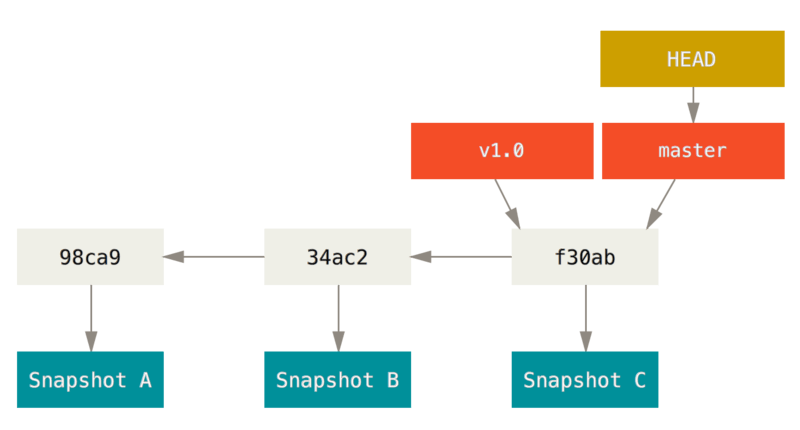
\includegraphics[scale=0.30]{How_Git_Branches_Work-1.png}
	\end{figure}
	\begin{itemize}
		\item{Branches can be created with \textbf{git branch \textless{}branchname\textgreater{}}}
	\end{itemize}
\end{frame}

\begin{frame}
	\frametitle{Creating Branches}
	\begin{itemize}
		\item{The new branch points to the commit you are currently on}
		\item{\textbf{git branch testing}}
	\end{itemize}
	\begin{figure}
		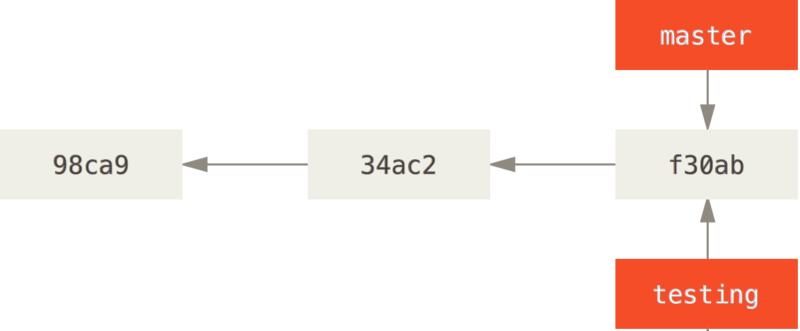
\includegraphics[scale=0.32]{Creating_Branches-0.png}
	\end{figure}
\end{frame}

\begin{frame}
	\frametitle{Creating Branches}
	\begin{itemize}
		\item{Git uses a special pointer to keep track of what the current branch is}
		\item{This pointer is called HEAD}
		\item{\textbf{git branch testing}}
	\end{itemize}
	\begin{figure}
		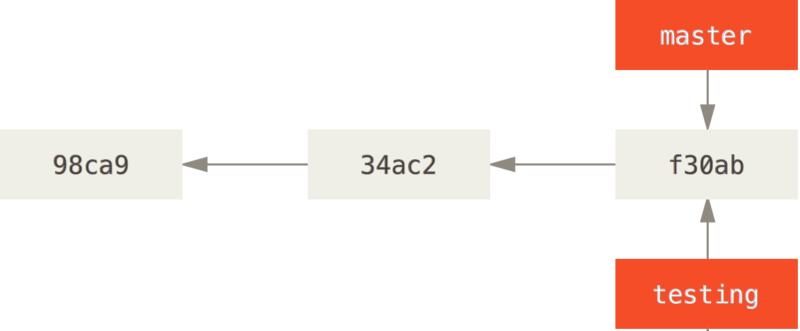
\includegraphics[scale=0.32]{Creating_Branches-0.png}
	\end{figure}
\end{frame}

\begin{frame}
	\frametitle{Switching Branches}
	\begin{itemize}
		\item{git branch only creates a new branch pointer, it doesn't switch to the branch}
		\item{To switch to another branch, use \textbf{git checkout \textless{}branchname\textgreater{}}}
		\item{\textbf{git checkout testing}}
	\end{itemize}
	\begin{figure}
		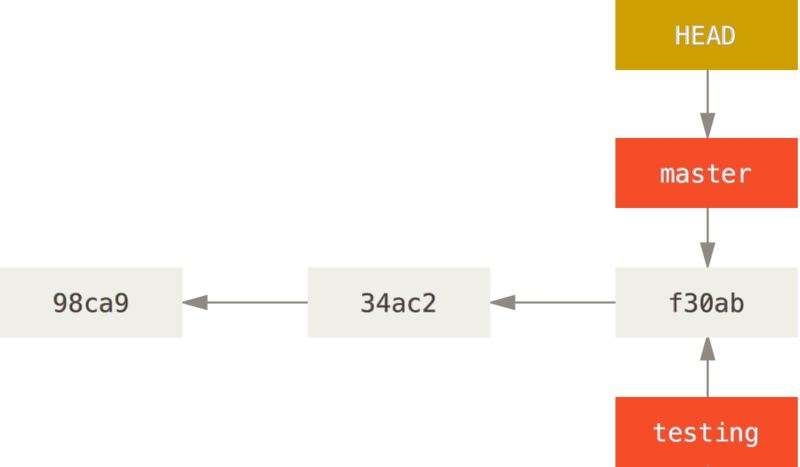
\includegraphics[scale=0.32]{Switching_Branches-0.png}
	\end{figure}
\end{frame}

\begin{frame}
	\frametitle{Switching Branches}
	\begin{itemize}
		\item{git branch only creates a new branch pointer, it doesn't switch to the branch}
		\item{To switch to another branch, use \textbf{git checkout \textless{}branchname\textgreater{}}}
		\item{\textbf{git checkout testing}}
	\end{itemize}
	\begin{figure}
		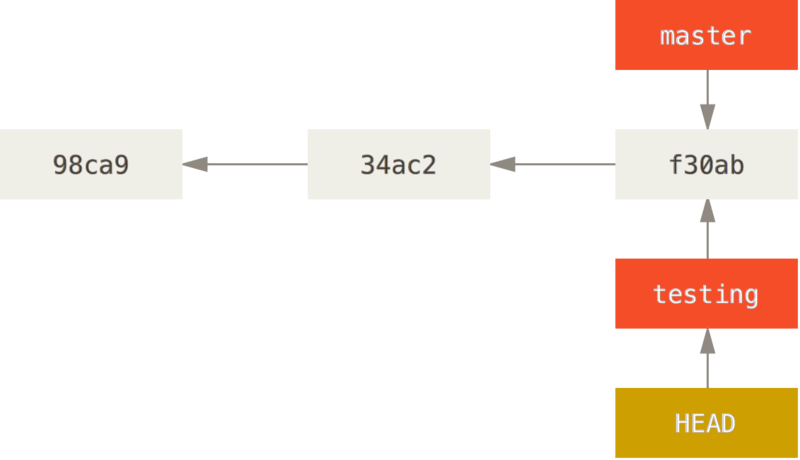
\includegraphics[scale=0.32]{Switching_Branches-1.png}
	\end{figure}
\end{frame}

\begin{frame}
	\frametitle{Switching Branches}
	\begin{itemize}
		\item{Can also just use  \textbf{git checkout -b \textless{}branchname\textgreater{}}}
	\end{itemize}
	\begin{figure}
		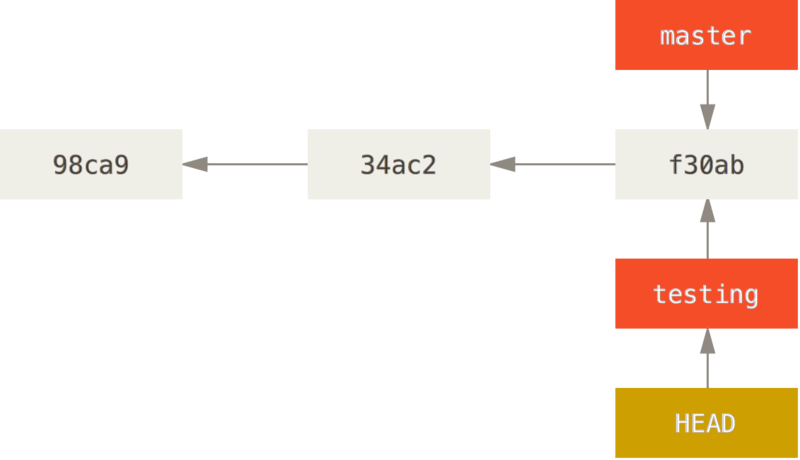
\includegraphics[scale=0.32]{Switching_Branches-1.png}
	\end{figure}
\end{frame}

\begin{frame}
	\frametitle{Diverging Branches}
	\begin{itemize}
		\item{You make a commit on the testing branch..}
	\end{itemize}
	\begin{figure}
		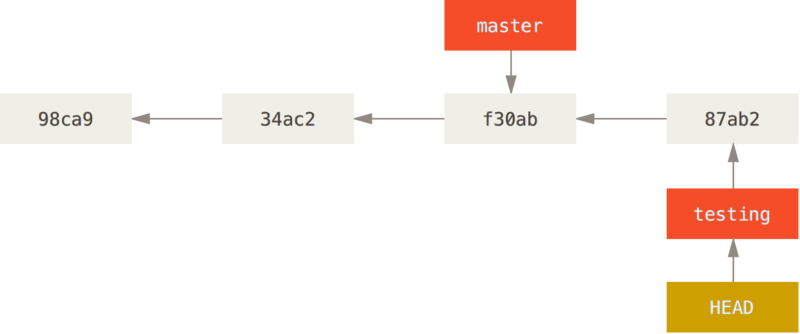
\includegraphics[scale=0.4]{Diverging_Branches-0.png}
	\end{figure}
\end{frame}

\begin{frame}
	\frametitle{Diverging Branches}
	\begin{itemize}
		\item{Then switch back to master with \textbf{git checkout master}..}
	\end{itemize}
	\begin{figure}
		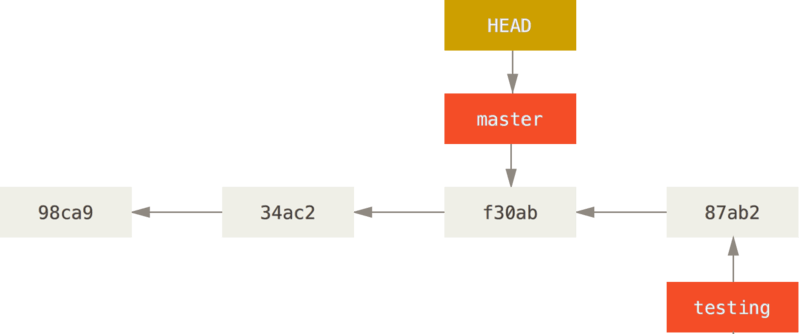
\includegraphics[scale=0.4]{Diverging_Branches-1.png}
	\end{figure}
\end{frame}

\begin{frame}
	\frametitle{Diverging Branches}
	\begin{itemize}
		\item{Then make a commit on master}
		\item{Now the history of master and testing has diverged}
	\end{itemize}
	\begin{figure}
		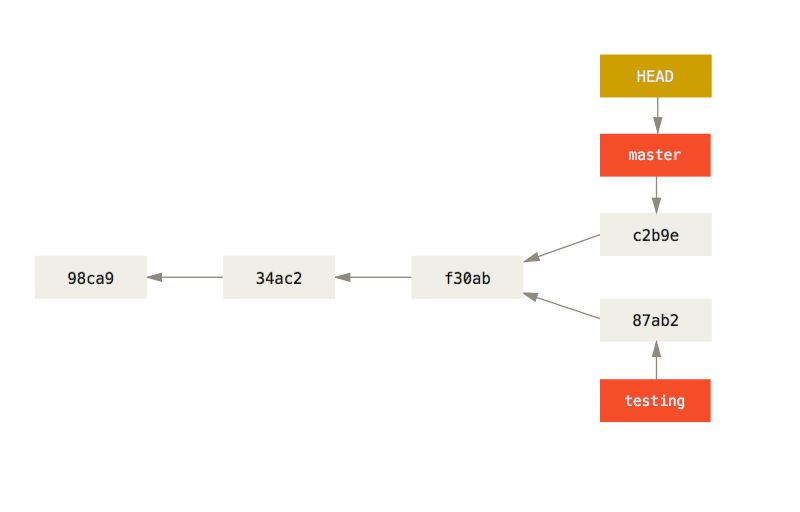
\includegraphics[scale=0.4]{Diverging_Branches-2.png}
	\end{figure}
\end{frame}

\begin{frame}
	\frametitle{Viewing the History with Branches}
	\begin{itemize}
		\item{\textbf{git log --all --oneline --graph}}
		\item{all: show all branches}
		\item{graph: visually indicate divergent history}
	\end{itemize}
	\begin{figure}
		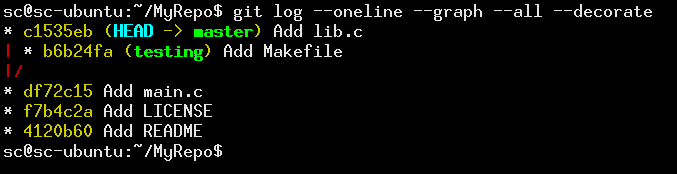
\includegraphics[scale=0.45]{Viewing_the_History_With_Branches-0.png}
	\end{figure}
\end{frame}

\begin{frame}
	\frametitle{Advantages of Branches in Git}
	\begin{itemize}
		\item{In Git, a branch is a file containing a 40-character SHA-1}
		\item{The SHA-1 is the checksum of the commit it points to}
		\item{Creating a new branch in Git = writing 41 bytes to a file}
	\end{itemize}
\end{frame}

\begin{frame}
	\frametitle{Merging Branches}
	\begin{itemize}
		\item{A common use case for branches is "feature branches"}
		\item{You create a new branch for a feature}
		\item{You do the commits for that feature on that branch only}
		\item{Once the feature is done, you merge the feature branch into master}
	\end{itemize}
\end{frame}

\begin{frame}
	\frametitle{Merging Branches}
	\begin{itemize}
		\item{Master branch and new branch "iss53" created}
	\end{itemize}
	\begin{figure}
		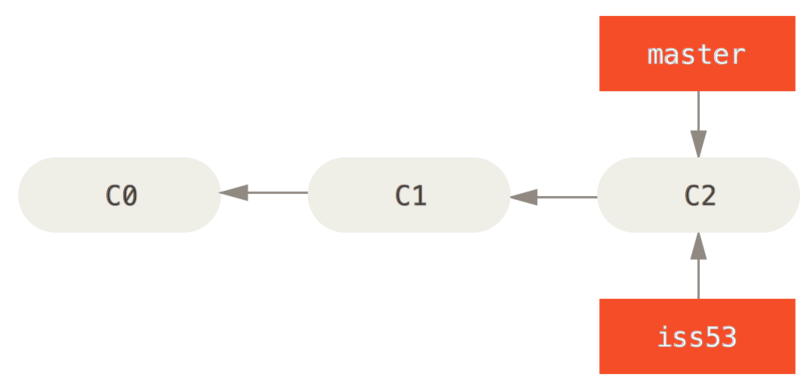
\includegraphics[scale=0.4]{Merging_Branches-0.png}
	\end{figure}
\end{frame}

\begin{frame}
	\frametitle{Merging Branches}
	\begin{itemize}
		\item{\textbf{git checkout iss53}}
		\item{Do some work and \textbf{git commit}}
	\end{itemize}
	\begin{figure}
		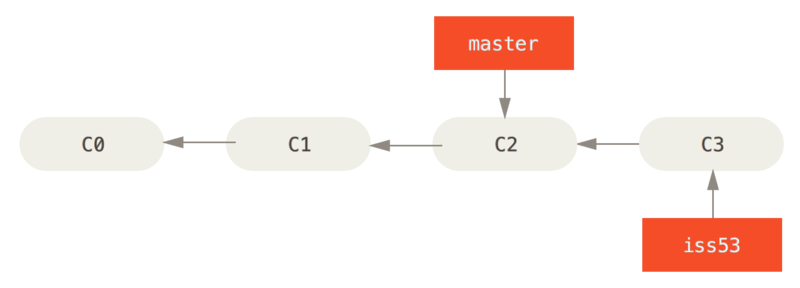
\includegraphics[scale=0.4]{Merging_Branches-1.png}
	\end{figure}
\end{frame}

\begin{frame}
	\frametitle{Merging Branches}
	\begin{itemize}
		\item{Notified of a bug on master branch}
		\item{\textbf{git checkout master}}
		\item{\textbf{git checkout -b hotfix}}
		\item{Write a fix and \textbf{git commit}}
	\end{itemize}
	\begin{figure}
		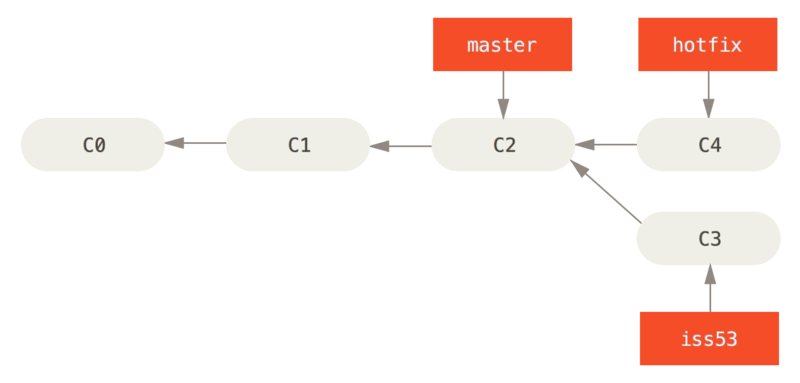
\includegraphics[scale=0.4]{Merging_Branches-2.png}
	\end{figure}
\end{frame}

\begin{frame}
	\frametitle{Merging Branches}
	\begin{itemize}
		\item{Hotfix doesn't exist on master unless we manually merge it}
		\item{To merge in Git, use \textbf{git merge \textless{}branch\textgreater{}}}
		\item{This merges \textless{}branch\textgreater{} into the current branch}
	\end{itemize}
	\begin{figure}
		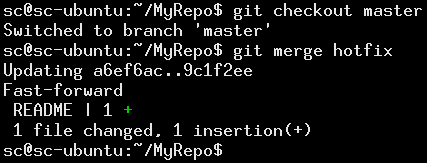
\includegraphics[scale=0.5]{Merging_Branches-3.png}
	\end{figure}
\end{frame}

\begin{frame}
	\frametitle{Merging Branches}
	\begin{itemize}
		\item{In this case, the merge is a "fast forward"}
		\item{This is because the hotfix pointer was directly ahead of master}
		\item{So the master pointer can simply be moved forward to hotfix}
	\end{itemize}
	\begin{figure}
		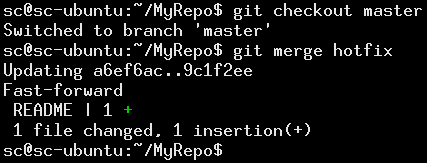
\includegraphics[scale=0.5]{Merging_Branches-3.png}
	\end{figure}
\end{frame}

\begin{frame}
	\frametitle{Merging Branches}
	\begin{itemize}
		\item{In this case, the merge is a "fast forward"}
		\item{This is because the hotfix pointer was directly ahead of master}
		\item{So the master pointer can simply be moved forward to hotfix}
	\end{itemize}
	\begin{figure}
		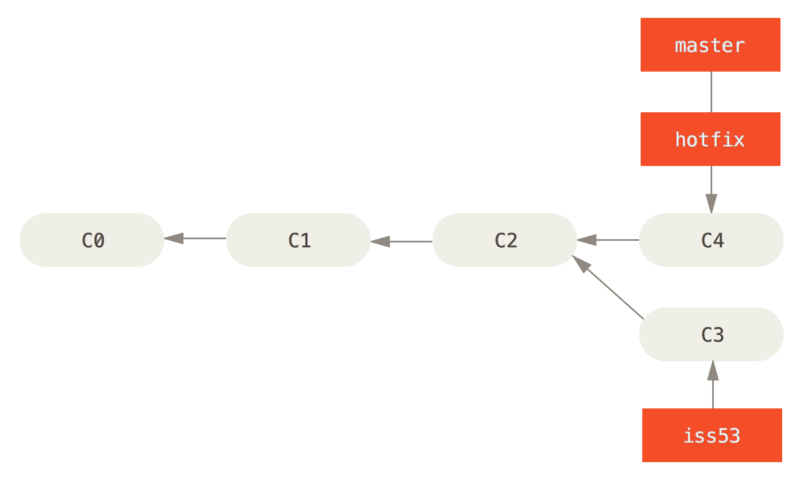
\includegraphics[scale=0.35]{Merging_Branches-4.png}
	\end{figure}
\end{frame}

\begin{frame}
	\frametitle{Merging Branches}
	\begin{itemize}
		\item{Once a branch has been finally merged you can delete it}
		\item{Do this with \textbf{git branch -d hotfix}}
		\item{This only deletes the pointer, the commits are safely on master}
	\end{itemize}
	\begin{figure}
		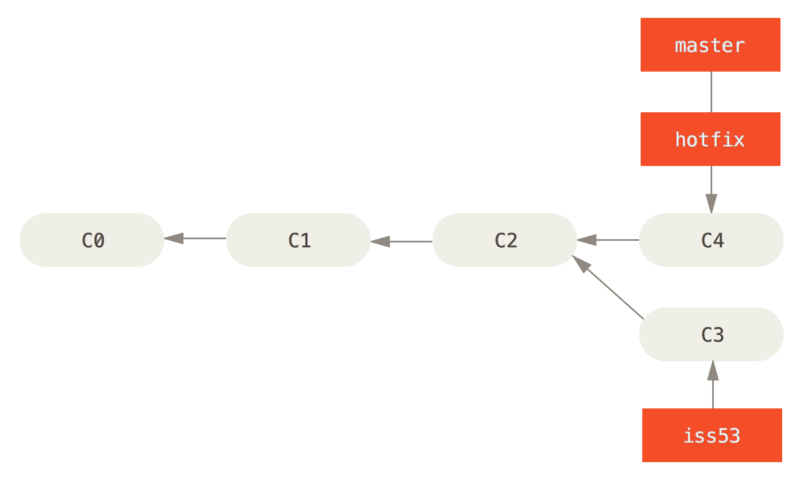
\includegraphics[scale=0.35]{Merging_Branches-4.png}
	\end{figure}
\end{frame}

\begin{frame}
	\frametitle{Merging Branches}
	\begin{itemize}
		\item{Now we switch back to iss53 branch and continue committing}
	\end{itemize}
	\begin{figure}
		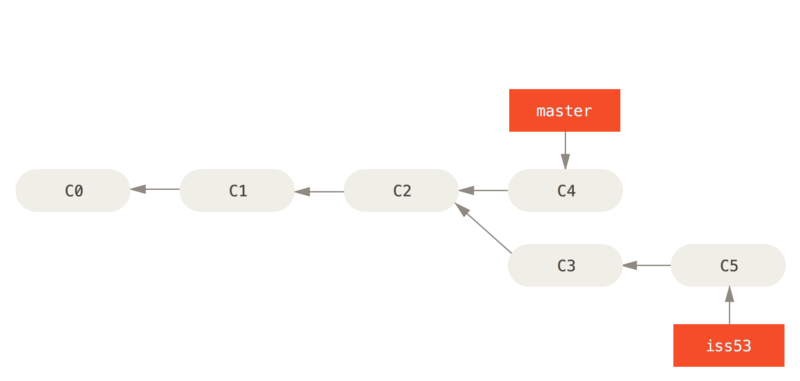
\includegraphics[scale=0.37]{Merging_Branches-5.png}
	\end{figure}
\end{frame}

\begin{frame}
	\frametitle{Merging Branches}
	\begin{itemize}
		\item{Once iss53 is complete, it can be merged into master}
	\end{itemize}
	\begin{figure}
		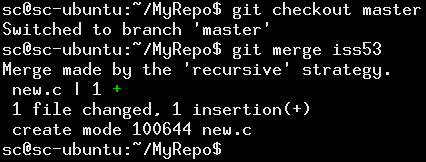
\includegraphics[scale=0.5]{Merging_Branches-6.png}
	\end{figure}
\end{frame}

\begin{frame}
	\frametitle{Merging Branches}
	\begin{itemize}
		\item{This merge wasn't a fast forward}
		\item{This is because the current commit in master isn't a direct ancestor of the top commit in iss53}
	\end{itemize}
	\begin{figure}
		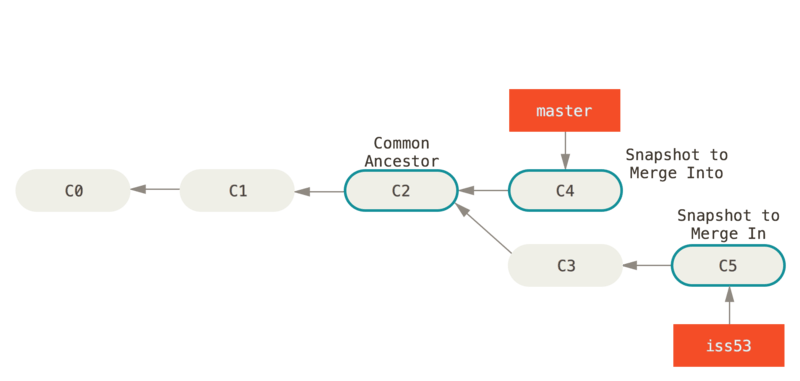
\includegraphics[scale=0.38]{Merging_Branches-7.png}
	\end{figure}
\end{frame}

\begin{frame}
	\frametitle{Merging Branches}
	\begin{itemize}
		\item{Git creates a new snapshot for this merge}
		\item{A new commit is create that points to it}
		\item{This is often called a "merge commit"}
		\item{This merge commit has two parents}
	\end{itemize}
	\begin{figure}
		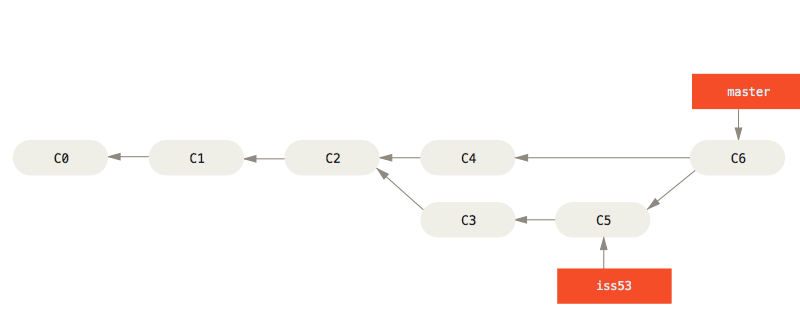
\includegraphics[scale=0.38]{Merging_Branches-8.png}
	\end{figure}
\end{frame}

\begin{frame}
	\frametitle{Merge Conflicts}
	\begin{itemize}
		\item{Not all merges go so smoothly}
		\item{If the top snapshot on each branch have different versions of the same file a merge conflict occurs}
	\end{itemize}
	\begin{figure}
		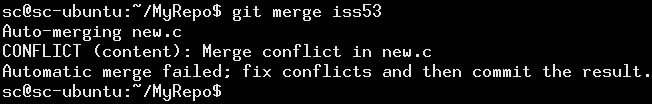
\includegraphics[scale=0.38]{Merging_Branches-9.png}
	\end{figure}
\end{frame}

\begin{frame}
	\frametitle{Merge Conflicts}
	\begin{itemize}
		\item{Not all merges go so smoothly}
		\item{If the top snapshot on each branch have different versions of the same file a merge conflict occurs}
	\end{itemize}
	\begin{figure}
		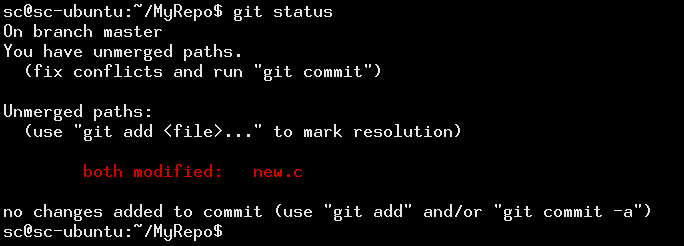
\includegraphics[scale=0.38]{Merging_Branches-10.png}
	\end{figure}
\end{frame}

\begin{frame}
	\frametitle{Merge Conflicts}
	\begin{itemize}
		\item{To resolve, open the conflicting file(s) in your editor}
		\item{Manually resolve the conflicts}
		\item{Git labels the conflicting segments of the file}
		\item{In this case, pick one version and delete the other}
	\end{itemize}
	\begin{figure}
		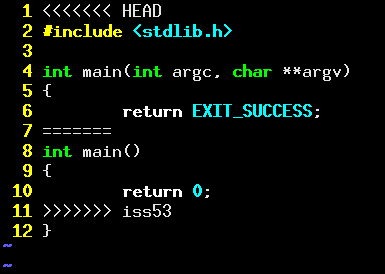
\includegraphics[scale=0.4]{Merging_Branches-11.png}
	\end{figure}
\end{frame}

\begin{frame}
	\frametitle{Merge Conflicts}
	\begin{itemize}
		\item{Once the files have been edited to resolve the conflicts:}
		\item{Stage the files}
		\item{\textbf{git commit}}
	\end{itemize}
	\begin{figure}
		\includegraphics[scale=0.4]{Merging_Branches-12.png}
	\end{figure}
\end{frame}

\begin{frame}
	\frametitle{Branch Management}
	\begin{itemize}
		\item{List branches with top commit on each: \textbf{git branch -v}}
		\item{List branches that are merged into current branch: \textbf{git branch --merged}}
		\item{List unmerged branches: \textbf{git branch --no-merged}}
	\end{itemize}
\end{frame}

\begin{frame}
	\frametitle{Rebasing}
	\begin{itemize}
		\item{Rebasing is another way of integrating changes from one branch into another}
		\item{In some situations it's better than merging, in some it's worse, and in some you shouldn't do it at all}
	\end{itemize}
\end{frame}

\begin{frame}
	\frametitle{Rebasing}
	\begin{figure}
		\includegraphics[scale=0.4]{Rebasing-0.png}
	\end{figure}
\end{frame}

\begin{frame}
	\frametitle{Rebasing}
	\begin{figure}
		\includegraphics[scale=0.4]{Rebasing-1.png}
	\end{figure}
\end{frame}

\begin{frame}
	\frametitle{Rebasing}
	\begin{itemize}
		\item{Can use rebasing to keep the history linear}
		\item{Take the patch introduced in C4 and reapply it on top of C3}
		\item{Avoids a merge commit}
	\end{itemize}
	\begin{figure}
		\includegraphics[scale=0.4]{Rebasing-2.png}
	\end{figure}
\end{frame}

\begin{frame}
	\frametitle{Rebasing}
	\begin{itemize}
		\item{Can use rebasing to keep the history linear}
		\item{Take the patch introduced in C4 and reapply it on top of C3}
		\item{Avoids a merge commit}
	\end{itemize}
	\begin{figure}
		\includegraphics[scale=0.4]{Rebasing-3.png}
	\end{figure}
\end{frame}

\begin{frame}
	\frametitle{Rebasing}
	\begin{itemize}
		\item{Now the history has been linearised with regard to the two branches}
		\item{Just need to update master's branch pointer}
	\end{itemize}
	\begin{figure}
		\includegraphics[scale=0.4]{Rebasing-4.png}
	\end{figure}
\end{frame}

\begin{frame}
	\frametitle{Rebasing}
	\begin{itemize}
		\item{Now the history has been linearised with regard to the two branches}
		\item{Just need to update master's branch pointer}
	\end{itemize}
	\begin{figure}
		\includegraphics[scale=0.4]{Rebasing-5.png}
	\end{figure}
\end{frame}

\begin{frame}
	\frametitle{Rebasing}
	\begin{itemize}
		\item{Now the history has been linearised with regard to the two branches}
		\item{Just need to update master's branch pointer}
	\end{itemize}
	\begin{figure}
		\includegraphics[scale=0.4]{Rebasing-5.png}
	\end{figure}
\end{frame}

\end{document}
